\documentclass[border=10pt]{standalone}
\usepackage[svgnames]{xcolor}
\usepackage{amsmath}
\usepackage{pgfplots}
\pgfplotsset{compat=newest}
\usepackage[sfdefault]{FiraSans}
\usepackage{FiraMono}
\renewcommand*\familydefault{\sfdefault}
\begin{document}
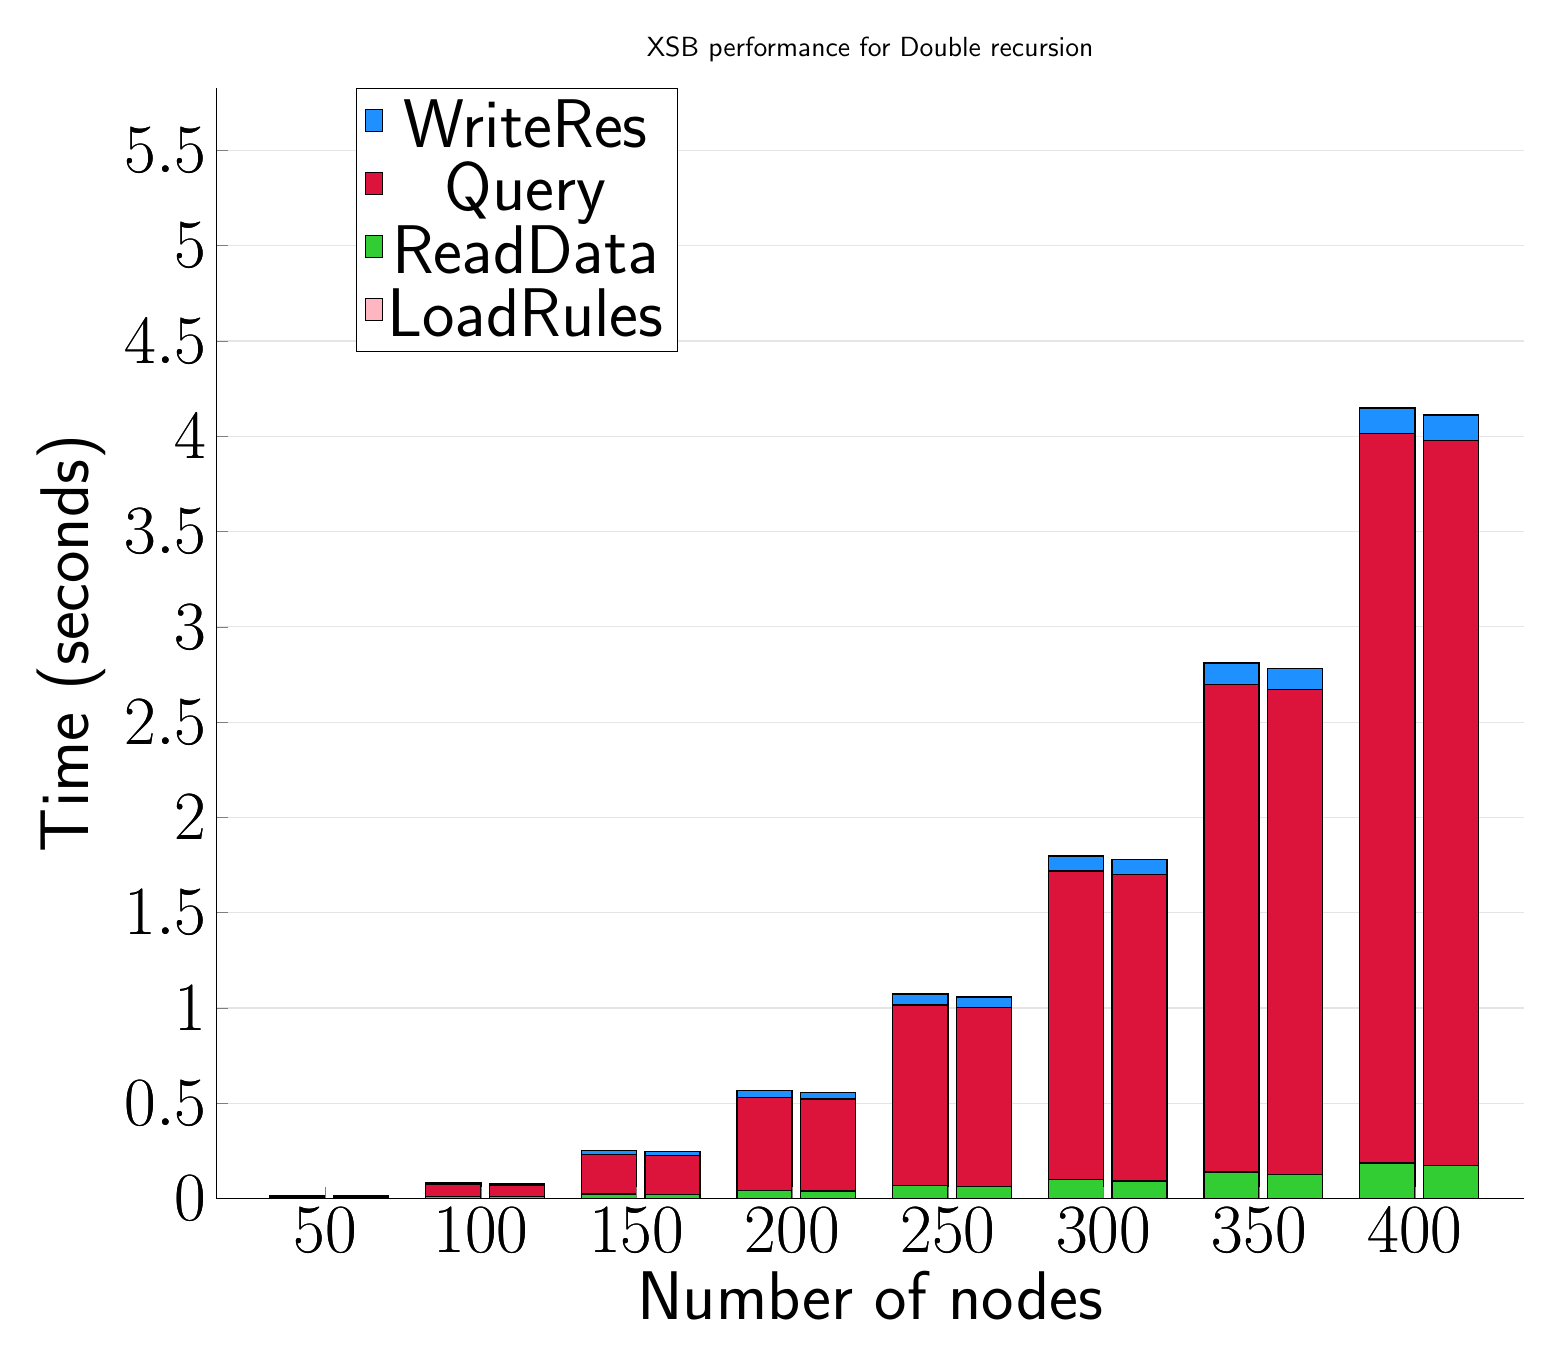
\begin{tikzpicture}
	\begin{axis}[
			ybar stacked,
			title={XSB performance for Double recursion},
			bar shift=-10pt,
			width=1.5\textwidth,
			bar width=0.7cm,
			ymajorgrids, tick align=inside,
			major grid style={draw=gray!20},
			xtick=data,
			ymin=0, ymax=5.828503680229188,
			axis x line*=bottom,
			axis y line*=left,
			enlarge x limits=0.1,
			legend style={
					at={(0.23, 1)},
					anchor=north,
					legend columns=1,
					font=\Huge,
				},
			ylabel={Time (seconds)},
			xlabel={Number of nodes},
			label style={font=\Huge},
			tick label style={font=\Huge},
		]
		\addlegendimage{fill=DodgerBlue, draw=black, line width=0.2pt}
		\addlegendentry{WriteRes}
		\addlegendimage{fill=Crimson, draw=black, line width=0.2pt}
		\addlegendentry{Query}
		\addlegendimage{fill=LimeGreen, draw=black, line width=0.2pt}
		\addlegendentry{ReadData}
		\addlegendimage{fill=LightPink, draw=black, line width=0.2pt}
		\addlegendentry{LoadRules}
		\addplot +[fill=LightPink, draw=black, line width=0.5pt] coordinates {
				(50, 0.0010901689529418932)
				(100, 0.0010718107223510753)
				(150, 0.001024174690246582)
				(200, 0.001073884963989259)
				(250, 0.001110482215881349)
				(300, 0.0011221885681152338)
				(350, 0.001091432571411132)
				(400, 0.0011713981628417968)
			};
		\addplot +[fill=LimeGreen, draw=black, line width=0.5pt] coordinates {
				(50, 0.0026510953903198234)
				(100, 0.010034990310668946)
				(150, 0.0229175090789795)
				(200, 0.042190814018249534)
				(250, 0.06754691600799559)
				(300, 0.09919433593750004)
				(350, 0.13749871253967288)
				(400, 0.18533658981323242)
			};
		\addplot +[fill=Crimson, draw=black, line width=0.5pt] coordinates {
				(50, 0.007768607139587403)
				(100, 0.061330556869506836)
				(150, 0.207903003692627)
				(200, 0.4871938943862915)
				(250, 0.9480813264846801)
				(300, 1.619144654273986)
				(350, 2.5606039285659774)
				(400, 3.8285036802291876)
			};
		\addplot +[fill=DodgerBlue, draw=black, line width=0.5pt] coordinates {
				(50, 0.0027324199676513673)
				(100, 0.009842061996459973)
				(150, 0.020610475540161204)
				(200, 0.0359254837036133)
				(250, 0.0563139677047728)
				(300, 0.07917466163635398)
				(350, 0.11159384250641113)
				(400, 0.134348225593565)
			};
	\end{axis}
	\begin{axis}[
			ybar stacked,
			bar shift=13pt,
			width=1.5\textwidth,
			bar width=0.7cm,
			ymajorgrids, tick align=inside,
			major grid style={draw=none},
			xtick=data,
			ymin=0, ymax=5.828503680229188,
			axis x line*=none,
			axis y line*=none,
			enlarge x limits=0.1,
			label style={font=\Huge},
			tick label style={font=\Huge},
		]
		\addplot +[fill=LightPink, draw=black, line width=0.5pt] coordinates {
				(50, 0.0006185000000000001)
				(100, 0.0006165999999999998)
				(150, 0.0005919)
				(200, 0.0006088000000000002)
				(250, 0.0006273000000000003)
				(300, 0.0006271000000000004)
				(350, 0.0006229)
				(400, 0.0006426000000000003)
			};
		\addplot +[fill=LimeGreen, draw=black, line width=0.5pt] coordinates {
				(50, 0.0022533)
				(100, 0.008968100000000001)
				(150, 0.020756)
				(200, 0.0381426)
				(250, 0.061549900000000005)
				(300, 0.09132929999999999)
				(350, 0.126653)
				(400, 0.171447)
			};
		\addplot +[fill=Crimson, draw=black, line width=0.5pt] coordinates {
				(50, 0.0076763)
				(100, 0.0606592)
				(150, 0.2059825)
				(200, 0.4827714)
				(250, 0.940304)
				(300, 1.6085115)
				(350, 2.5452947999999997)
				(400, 3.8049542)
			};
		\addplot +[fill=DodgerBlue, draw=black, line width=0.5pt] coordinates {
				(50, 0.0024341000000000002)
				(100, 0.0092322)
				(150, 0.019923299999999998)
				(200, 0.0353161)
				(250, 0.0558608)
				(300, 0.0779628)
				(350, 0.10887960000000008)
				(400, 0.13417229999999997)
			};
	\end{axis}
\end{tikzpicture}

\end{document}
